\documentclass[UTF8,9pt]{ctexart}
\usepackage{../../template/homeworkTEMP/hw}
\setcounter{secnumdepth}{0}
    \title{The 3rd Homework of Theoretical Mechanics} 
\begin{document} 
    \maketitle 
    \section{Q1}
        \putfig{0.4}{2.png}
        该瞬时后一段时间,凸轮运动了$x$。设杆支点距地面$h$,该瞬时$\t=\t_0$, 则:
        $$h=\f{l_{AC}}{\sin\t_0}=\f{R}{\sin\t_0}=x\cot\t+\f{R}{\sin\t}$$
        $$\implies x\cos\t+R=h\sin\t$$
        两边求导:
        $$\dot{x}\cos\t-x\sin\t\dot{\t}=h\cos\t\dot{\t}$$
        $$\implies \dot{\t}=\f{\dot{x}}{h+x\tan\t}$$ 
        $$\ddot{\t}=\dt{\dot{\t}}=\f{a(h+x\tan\t)-v(v\tan\t+x\sec^2\t)}{(h+x\tan\t)^2}$$
        该瞬时$x=0$,与$h=\f{R}{\sin\t_0}$代入上面两式:
        $$\dot\t=\f{v\sin\t_0}{R}$$
        $$\ddot\t=\f{a\sin\t_0}{R}-\f{v^2\sin^3\t_0}{R^2\cos\t_0}$$
    \section{Q2} 
        以正南为x方向,正东为y方向,竖直向上为z方向建立坐标系,此时:
        $$\bm{\omega}=(-\omega\cos\lambda,0,\omega\sin\lambda)$$
        $$\bm{v}(0)=(0,V\cos\alpha,V\sin\alpha)$$
        $$a=g-2 \bm{\omega} \times \bm{v} \ \ \text{(忽略}\omega^2\text{项)}$$
        $$\Rightarrow \left\{\begin{array}{rll}
            a_x=&2\omega\sin\lambda v_y & v_x(0)=0\\ 
            a_y=&-2(\omega\cos\lambda v_z+\omega\sin\lambda v_x)&v_y(0)=V\cos\alpha\\
            a_z=&-g+2\omega\cos\lambda v_y &v_z(0)=V\sin\alpha
        \end{array}\right.$$
        积分:
        $$\Rightarrow \left\{\begin{array}{rl}
            v_x=&2\omega\sin\lambda y \\ 
            v_y=&-2(\omega\cos\lambda z+\omega\sin\lambda x)+V\cos\alpha\\
            v_z=&-gt+2\omega\cos\lambda x +V\sin\alpha
        \end{array}\right.$$
        代入并舍弃$\omega^2$项可以得到:
        $$\Rightarrow \left\{\begin{array}{rll}
            a_x=&2\omega\sin\lambda V\cos\alpha\\ 
            a_y=&-2\omega\cos\lambda (-gt +V\sin\alpha)\\
            a_z=&-g+2\omega\cos\lambda V\cos\alpha
        \end{array}\right.$$
        观察发现,物体在$x,z$方向加速度为常数。运动时间为2倍上升时间:
        $$t=2t_0 \simeq 2\f{V\sin\alpha}{g}$$
        $$\implies x=\int v_x \d t=\iint 2\omega\sin\lambda V\cos\alpha (\d t)^2$$
        $$=\omega\sin\lambda V\cos\alpha t^2=\f{4V^3}{g^2}\sin^2\alpha\omega\sin\lambda\cos\alpha$$
    \section{Q3}
        建立固连在圆环上的坐标系如图:
        \begin{center}
            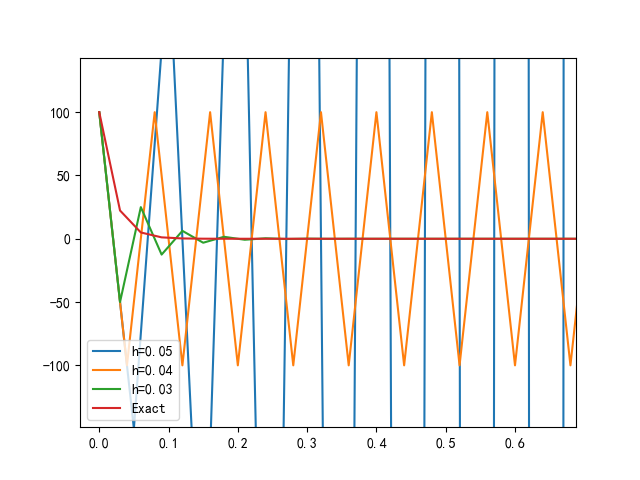
\includegraphics[scale=0.2]{1.png}\\ 
        \end{center}
        $$\bm{a'}=\omega^2 2a\cos\theta\bm{e_r}-2\bm{\omega} \times \bm{v}'$$
        $$=(\omega^2 2a\cos^2\theta+2\omega \times v')\bm{e_o}-\omega^2 2a\cos\theta\sin\theta\bm{e_t}$$
        其中,切向加速度为:
        $$a_t=-2a\omega^2 \cos\theta\sin\theta=-a\omega^2\sin2\theta=a\ddot{\theta}$$
        $$\Rightarrow \ddot{\theta}=-\omega^2\sin2\theta$$
    \section{Q4}
        \subsection{i}
            当$\theta$减小$\delta\theta$,\\
            重力做功:
            $$W_G=W(a+b)(\sin\theta-\sin(\theta-\delta\theta))=W(a+b)\cos\theta \delta\theta$$
            弹力做功:
            $$W_E=\ff{2}k(2b\cos\theta-l)^2-\ff{2}k(2b\cos\theta -l+ 2b\sin\theta \delta\theta)^2=-2kb \sin \theta (2b\cos\theta -l) \delta\theta$$
            平衡时$W_G+W_E=0$,即:
            $$2kb \sin \theta (2b\cos\theta -l) \delta\theta=W(a+b)\cos\theta \delta\theta$$
            $$ \Rightarrow \theta=\arctan\f{w(a+b)}{2kb(2b\cos\theta-l)}$$
        \subsection{ii}
            设棒的全长为$l$,其质心离碗面距离为$h$,棒与水平面夹角为$\alpha$,
            $$\cos\alpha=\f{c}{2r}$$
            $$\sin\alpha=\f{h}{c-l/2}$$  
            当棒稳定时,$\dd{h}{\alpha}=0$,
            $$\dd{h}{\alpha}=\dd{c}{\alpha}\sin\alpha+c\cos\alpha-\f{l}{2}\cos\alpha=0$$
            代入$\sin\alpha, \cos\alpha$可得:
            $$2r\left(1-\f{c^2}{4r^2}\right)=\left(c-\f{l}{2}\right)\f{c}{2r}$$
            $$\Rightarrow 2c-\f{4r^2}{c}=\f{l}{2}$$
            $$\Rightarrow l=\f{4(c^2-2r^2)}{c}$$
    \section{Q5}
        约束方程为:
        $$x^2+y^2+z^2=a^2 \Rightarrow 2x\delta x+2y\delta y + 2z\delta z=0$$
        重力做功:$$\delta W=mg\delta z$$
        根据lagrange乘子法:
        $$\delta W+ (2x\lambda\delta x+2y\lambda\delta y + 2z \lambda\delta z)=0$$
        $$\Rightarrow 2x\lambda\delta x+2y\lambda\delta y + (2z \lambda+mg)\delta z=0$$
        解得:
        $$
            \lambda=-\f{mg}{2z} \Rightarrow x=y=0
        $$
        因此平衡位置为:$(0,0,0),(0,0,2a)$,约束力为:
        $$R=\lambda\nabla f=-\f{mg}{2z} 2z\vec{k}=-mg\vec{k}$$
\end{document}